\chapter{System evaluation}
\label{System_evaluation}
%introduction - %current state
In the previous chapter an algorithm has been proposed, which should be capable of classifying a set of consecutive samples into two groups: Activity detected or no activity detected. The algorithm is however dependent on several parameters which have not been determined yet. The goal of this chapter is to find a set of parameters for the algorithm and evaluate the system using the algorithm tuned with those parameters.

This chapter starts with showing the test set-up which will be used to create a diverse dataset. This dataset will then be used to find parameters for the algorithm with which we evaluate the system. This chapter finishes with evaluating the performance of the system.

\section{Test set-up}
\label{dataset}
The test set-up used for evaluating and tuning the system can be seen in Figure \ref{fig:setup_a}. It shows the platform placed at 280cm above the ground in a room at night. Figure \ref{fig:signalsinestsetup} shows 15 seconds of received samples when the system was turned on. It can be seen that all described noise sources in section \ref{receivedsignals} where detected in the test environment.

Figure \ref{fig:setup_a} also shows three possible paths a pedestrian can walk. Path 1, the centre path, is placed directly under the light. Path 2 and 3 where placed at 30cm and 60cm from the centre path. The pedestrian was asked to wear one of the hoodies shown in Figure \ref{fig:setup_b} before traversing one of the paths. The different colours where used to ensure that the system was tested on various albedo's.

The ground where the pedestrian walked upon also varied. It was either a lacquered wooden floor or a blue carpet. The carpet on the floor produced a mostly diffuse reflection. The wooden floor produced a diffuse and spread reflection. These two floors were chosen to simulate how the system performs in different environments.

With the described set-up we created test-cases in the following manner:
\begin{enumerate}[itemsep=-1ex,topsep=0pt]
	\item Position a person at the beginning of a path.
	\item Start the gathering of samples and let the person wait for $\pm$ 35 seconds.
	\item After $\pm$ 35 seconds, the person starts walking
	\item When the person has reached the end of a path, stop the measurement.
\end{enumerate}
This procedure was repeated six times for each combination of floor material, path and hoodie colour, resulting in 180 unique test-cases. An example test-case can be seen in Figure \ref{TestScenario}. 

A test-case is split up in three sections. The first section (the first 25 seconds of data) serves to initialise the filters of the filter section and to fill the FIFO buffers used to calculate the moving $\sigma$ and moving $\mu$. After these 25 seconds the system can start detecting events. This is where section two starts. In this section, no events which should be detected by the algorithm are present. Then, after 10 to 15 seconds, section three begins when the person starts walking. In this section, the algorithm should trigger a detection.

\begin{figure}
	\centering     %%% not \center
	\subfigure[]{\label{fig:setup_a}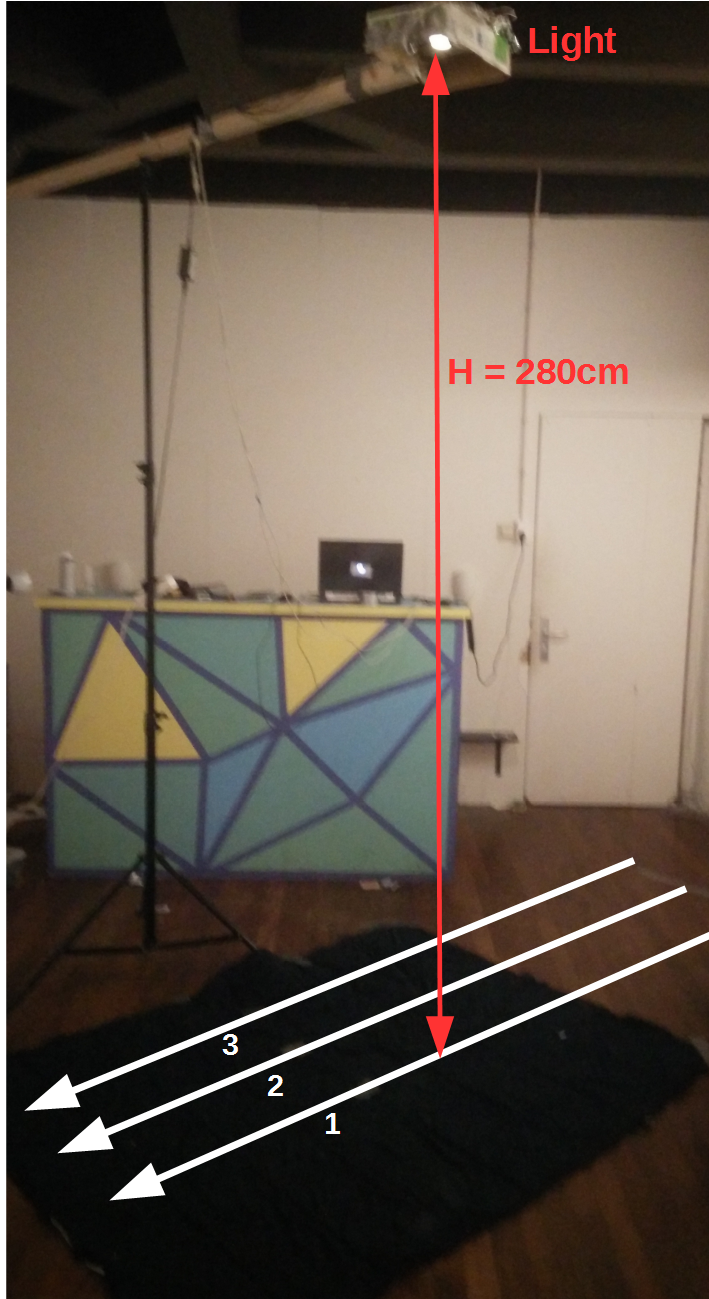
\includegraphics[width=50mm]{pics/Testsetup.png}}
	\subfigure[]{\label{fig:setup_b}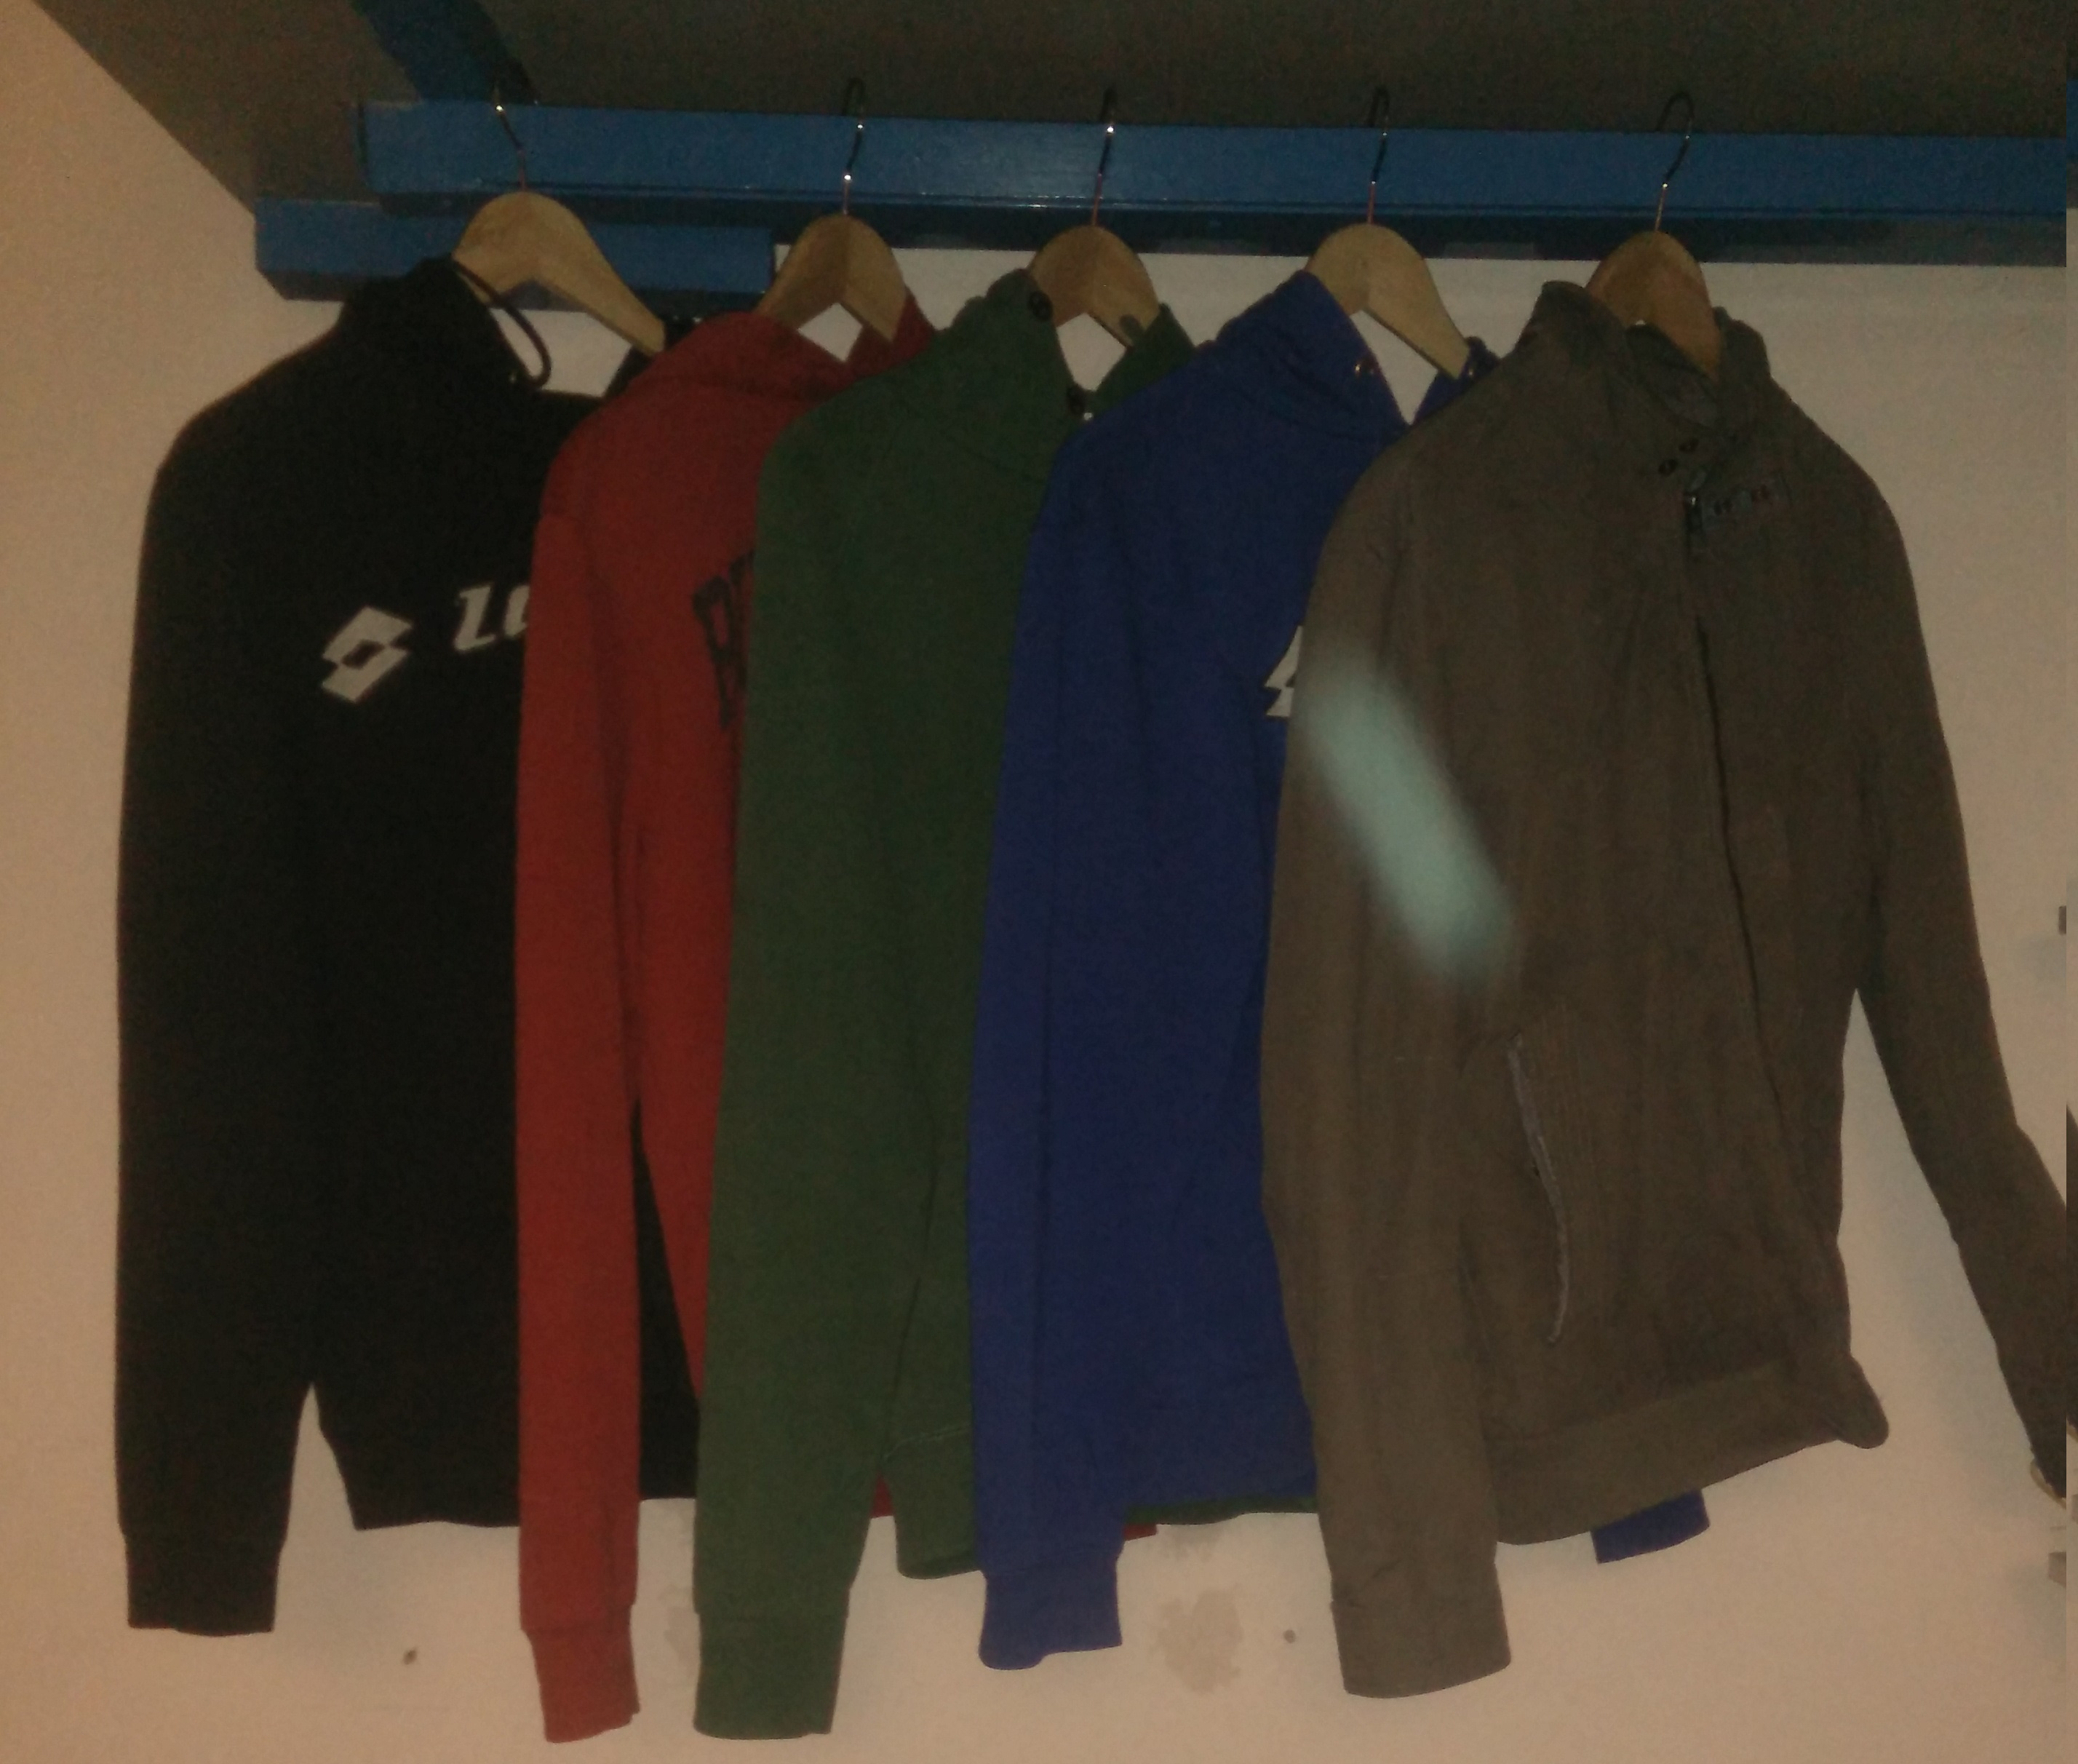
\includegraphics[width=70mm]{pics/Clothing.jpg}}
	\caption{(a) shows a picture of the test set-up with the blue carpet. The white arrows on the floor represent the three different paths the test subject walked over. The light is placed at a height of 2.8m. (b) shows the different clothing worn during the experiment (black, red, green, blue and grey).\label{fig:Testsetup}}
\end{figure}

\begin{figure}
	\centering     %%% not \center
	\subfigure[]{\label{fig:signals_Freq}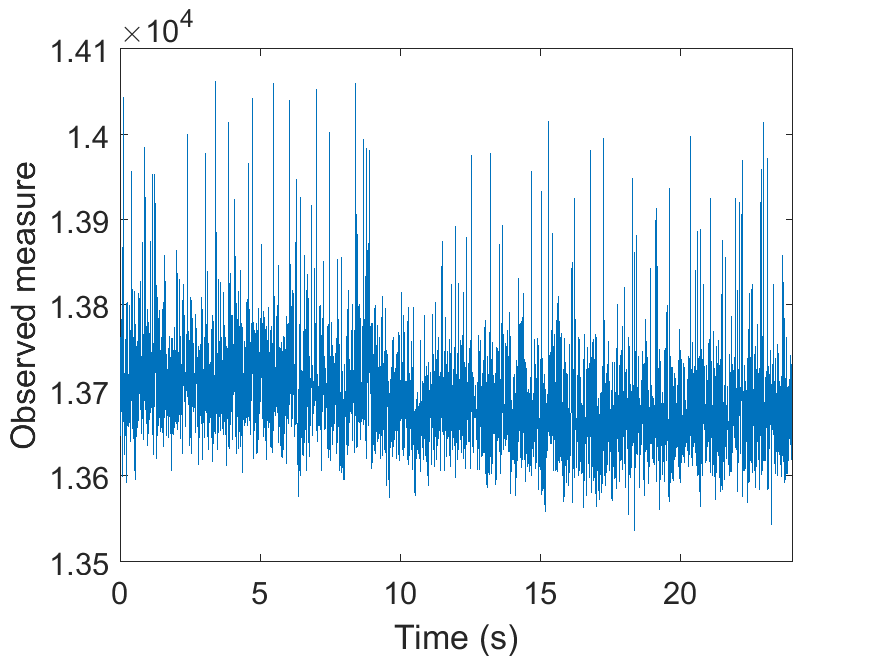
\includegraphics[width=60mm]{pics/Signal_Final_chp.png}}
	\subfigure[]{\label{fig:signals_raw}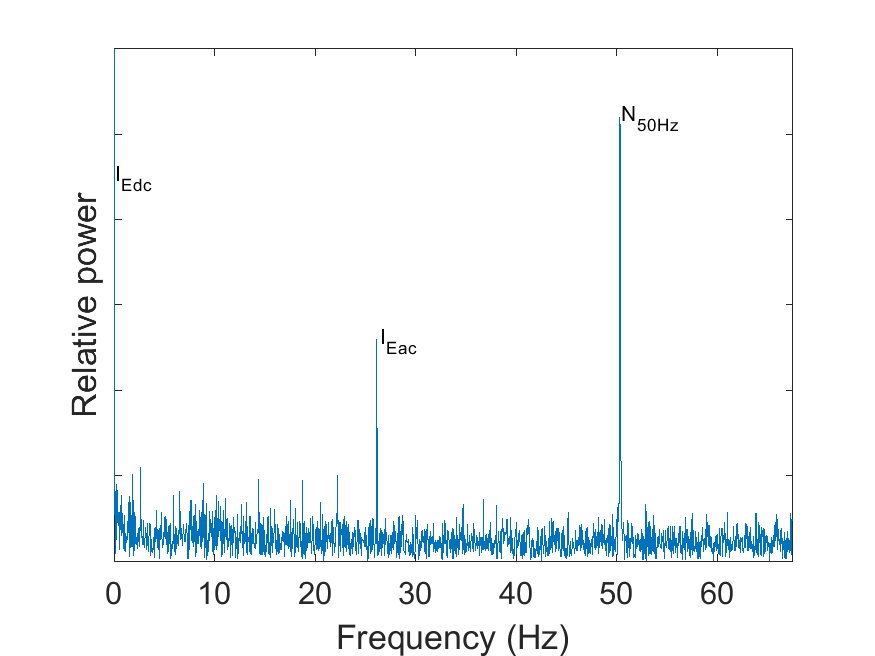
\includegraphics[width=60mm]{pics/Freqplot_Final_chp.png}}
	\caption{(a) shows the received signal and (b) shows the frequency of this signal. $I_{Eac}$ and $N_{50Hz}$ are best seen in figure (b). $I_{Edc}$ is best observed in (a) (the slowly dropping signal).\label{fig:signalsinestsetup}}
\end{figure}

\begin{figure}
	\centering     %%% not \center
	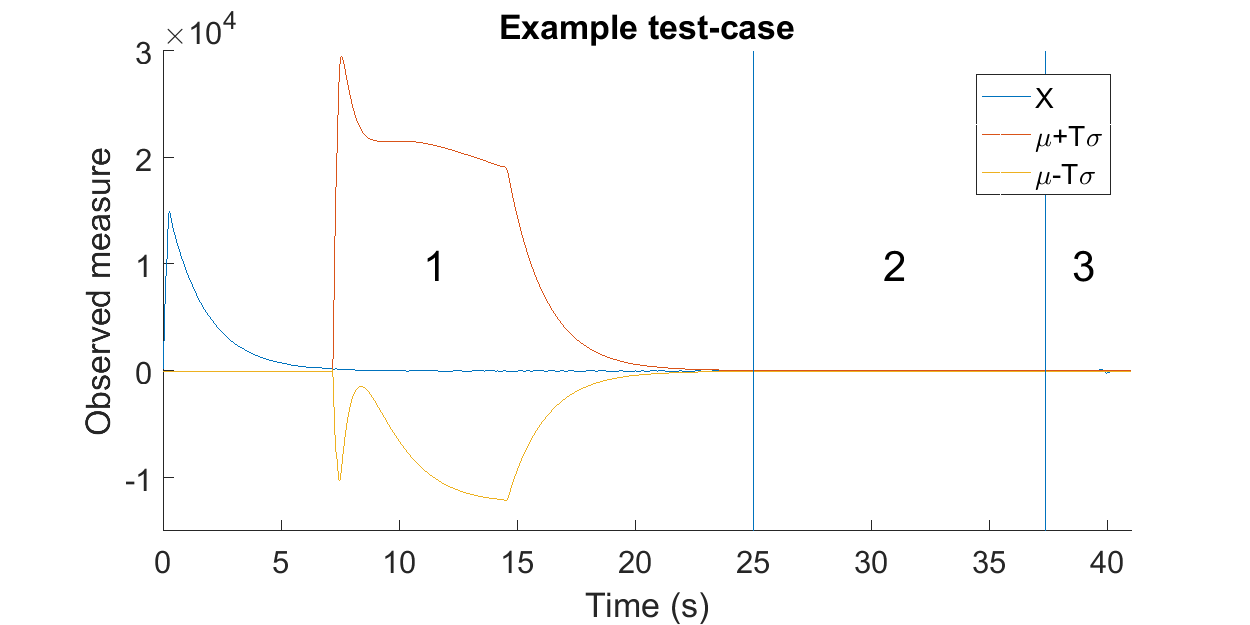
\includegraphics[width=\textwidth]{pics/Examplescenario.png}
	\caption{An example scenario with the tree sections marked. The first section is used to initialise the filters, moving mean and moving standard deviation. The second section is use to check for false positives. The first section is used to check if the event gets detected properly. \label{TestScenario}}
\end{figure}

\section{Algorithm parameters}
A genetic algorithm (GA) was used to find parameters fo the algorithm. GA's are commonly used to generate high-quality solutions to optimization and search problems. In this case, we need to find good settings for the algorithm.

A GA needs two things to work. The first is a way to summarise a solution as a \textit{gene}. In our case, a gene is simply a set of numbers which represent the parameters of the algorithm. The range of allowed inputs can be seen in Table \ref{tbl:genes}.

\begin{table}[]
	\centering
	\begin{tabular}{l|cccccc}
		& d & m & l  & L  & T  & k  \\ \hline
		Min & 0 & 1 & 1  & 1  & 1  & -1 \\
		Max & 1000 & 1000 & 10 & 10 & 10 & 1 
	\end{tabular}
	\caption{Overview of the possible input genes for the genetic algorithm.\label{tbl:genes}}
\end{table}

The second thing a GA needs to work is a fitness function. This function evaluates the input gene and scores it based on its performance. In our case, we want a gene representing an algorithm, which detects persons passing by while not triggering when nobody passes by. This can be achieved by having the fitness function evaluate a dataset $S$ and counting the amount of test-cases where it correctly and incorrectly detects the pedestrians. The final fitness can be calculated with equation \ref{eq:ff}, where $TP$ is the amount of correct detections in the observed dataset, $FP$ is the amount of false detections in the observed dataset and $N$ represents the amount of test-cases in the dataset.

\begin{equation}
	Fitness = \frac{TP - FP}{N} \cdot 100\%
	\label{eq:ff}
\end{equation}

The described fitness function was used to train two separate algorithms. The first algorithm $ALG_1$ was found using dataset $S_1$, which contained the 90 test-cases created with the wooden floor. The second algorithm trained, $ALG_2$, was found using dataset $S_2$, which contained the 90 test-cases created with the carpet. The found algorithms can be seen in Table \ref{Found_settings}.

\begin{table}[]
	\centering
\begin{tabular}{l|llllll|l}
	              & d   & m   & l & L  & T   & k    & Fitness \\ \cline{1-8} 
	$ALG_1$       & 980 & 890 & 7 & 9  & 4.5 & 0.2  & 91\%    \\
	$ALG_2$       & 860 & 980 & 8 & 10 & 5.9 & -0.7 & 83\%
\end{tabular}
	\caption{The settings found with the genetic algorithm. $STD_1$ was trained with dataset $S_1$ and $STD_2$ was trained with dataset $S_2$.\label{Found_settings}}
\end{table}

\section{Evaluation}
The two found algorithms where evaluated against three different datasets: $S_1$, $S_2$ and $S_3$. $S_3$, is the union of $S_1$ and $S_2$, and contains all 180 test-cases. Results of this evaluation can be seen in Table \ref{tbl:Scoringresults}. We are aware that evaluating the algorithm with the dataset it was trained with gives biased results, but they were added for the sake of completeness. The most interesting sections of the table are marked blue. These sections show the results of testing $ALG_1$ on $S_2$ and $ALG_2$ on $S_1$. It can be seen that both algorithms seem to perform reasonably well as they achieve a fitness of over 75\%.

\begin{table}[]
	\hskip-2.7cm
\begin{tabular}{l|lll|lll|lll}
	& \multicolumn{3}{c|}{$S_1$}                                                                         & \multicolumn{3}{c|}{$S_2$}                                                                           & \multicolumn{3}{c}{$S_1 \cup S_2$} \\ \hline
	Algorithm & TP (\%)                           & FP (\%)                         & Fitness                      & TP (\%)                           & FP (\%)                           & Fitness                      & TP (\%)      & FP (\%)   & Fitness  \\ \hline
	$ALG_1$   & 86 (96\%)                         & 4 (4\%)                         & 91\%                         & \cellcolor[HTML]{BBDAFF}81 (90\%) & \cellcolor[HTML]{BBDAFF}11 (12\%) & \cellcolor[HTML]{BBDAFF}78\% & 167 (93\%)   & 15 (8\%)  & 84\%     \\
	$ALG_2$   & \cellcolor[HTML]{BBDAFF}84 (93\%) & \cellcolor[HTML]{BBDAFF}3 (3\%) & \cellcolor[HTML]{BBDAFF}90\% & 81 (90\%)                         & 6 (7\%)                           & 83\%                         & 165 (91\%)   & 9 (5\%)   & 87\%    
\end{tabular}
	\caption{Results of testing the found algorithms against all datasets.\label{tbl:Scoringresults}}
\end{table}

This method however, does not give a good representation of how the system performs in the real world, as the fitness score of an algorithm does not tell us how much energy is saved and how much of the bypassing persons are actually detected. A better way to gain insight in the performance of this system is with recall and the false positive ratio.

Recall, $R$, is defined in equation \ref{eq:precsion/recall} and gives us insight in how often the system fails to detect an object passing by. $R = 1$ means that all events are detected were $R = 0$ means that none of the pedestrians are detected. The false positive ratio, $FP_r$, is defined in equation \ref{eq:precsion/recall} and gives us insight in how often the system makes a false detection. Because it's known how much time we observe when we determine if a false positive occurs, we can calculate the chance on a false positive per minute with equation \ref{eq:FPratio}.

If we evaluate the algorithms with these metrics, we see that $ALG_1$ has a 18\% chance on a false positive every minute and $ALG_2$ a 54\% chance. These numbers show that the system, with the current algorithm settings, makes too much mistakes and won't be usable to save energy. It is however possible to manually adjust the found parameters to better suit our system.

\begin{equation}
\label{eq:precsion/recall}
Recall = R = \frac{TP}{TP + FN}
\quad
FP_{r} = \frac{FP}{FP+TN}
\end{equation}

\begin{equation}
\label{eq:FPratio}
P_{FP/minute} = 1 - \left(1 - \frac{FP}{FP+TN}\right)^{6t}
\end{equation}

\begin{figure}
	\centering     %%% not \center
	\subfigure[]{\label{fig:STDs1_s2}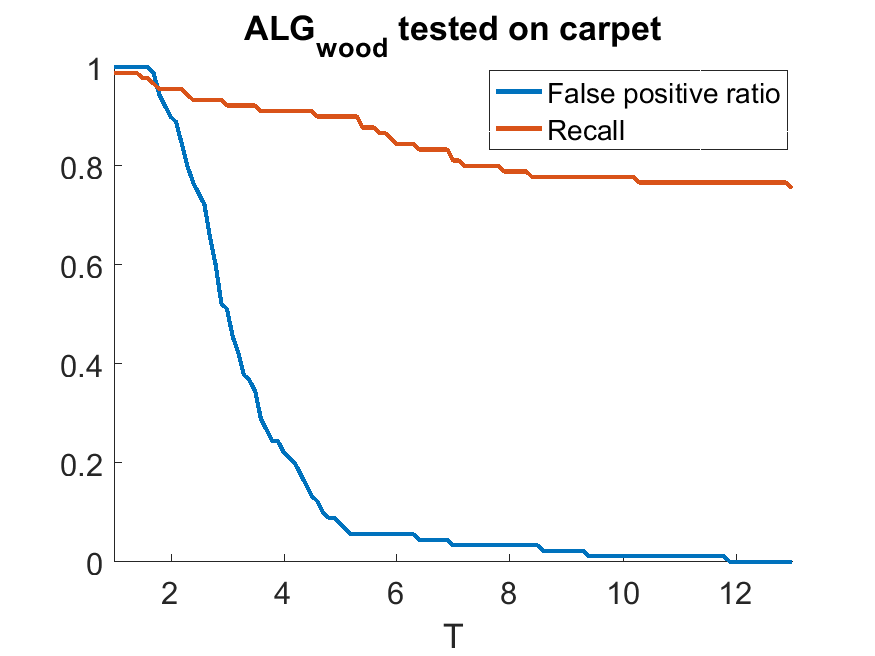
\includegraphics[width=60mm]{pics/STDs1_s2.png}}
	\subfigure[]{\label{fig:STDs2_s1}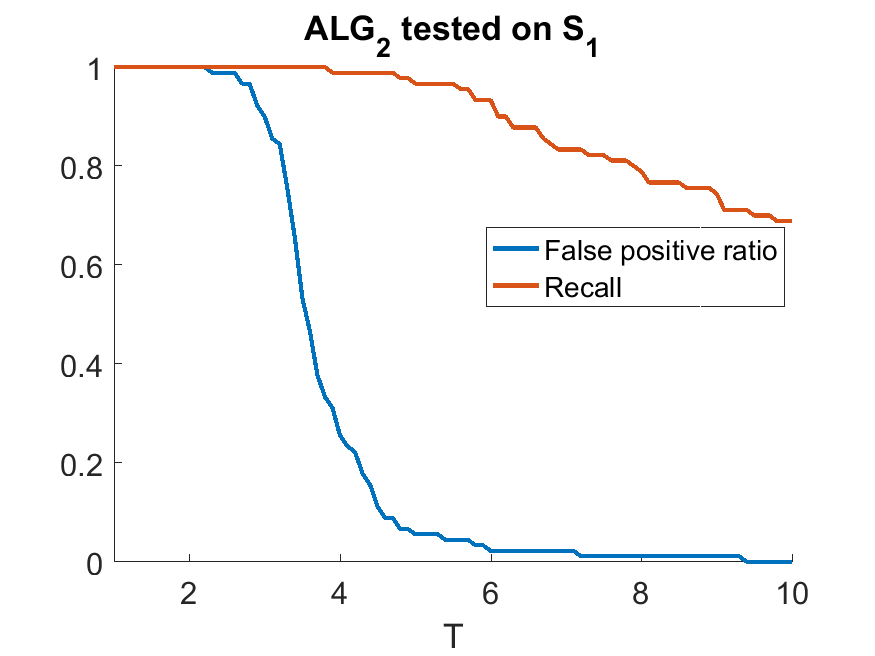
\includegraphics[width=60mm]{pics/STDs2_s1.png}}
	\caption{The false positive ratio and recall plotted as a function of $T$, for both created algorithms. \label{STDx_vs_Sx}}
\end{figure}

The easiest way to manually adjust the algorithm is by changing the value of $T$. $T$ directly influences the detection threshold. Raising $T$ will by definition, decrease the amount of false positives (lowering $FP_r$) and true positives (lowering recall) we detect. Two plots, showing $R$ and $FP_r$ as a function of $T$ for both algorithms can be seen in Figure \ref{STDx_vs_Sx}. 

In these plots it can be seen $FP_r$ drops fairly fast if $T$ increases, until $FP_r$ reaches $0.1$. From this point, $T$ needs to increase a lot, to further increase $FP_r$ significantly. This is because the false positives in these test-cases are not caused by the previously described noise sources but by artefacts occurring in the test data. One of such artefacts is shown in Figure \ref{fig:resforfailure} at $t = 32s$.

These artefacts are caused by slight fluctuations in the power supply of the flash receiver. This part of the system is powered by an USB port of the analyser. Slight voltage drops in the USB ports are common but usually no problem as the changes are minimal. If they get amplified 5600 times however, they become visible and will influence the measurements of the photodiode. this problem could be solved by powering the system with a battery or a very stable power supply. This is however no longer possible for this project due to time constraints.

It is however still possible to ignore the artefacts by choosing an ideal value for $T$ with the help of Figure \ref{STDx_vs_Sx}. For example, if we want a system which does not trigger any false positives (e.g. $FP_r = 0$), then we have to choose $T = 12$ for $ALG_1$ and $T = 9.6$ for $ALG_2$. This leads to the detection results shown in Table \ref{tbl:P=1}. It can be seen that the detection ratio of persons walking directly under the light is good (90\% and 100\%), but the further we move away from the centre, the worse the detection ratio (recall) becomes.

\begin{table}[]
	\centering	
\begin{tabular}{l|ccc|lll}
	& \multicolumn{3}{c|}{$ALG_2(S_1) \rightarrow FP_r = 0$} & \multicolumn{3}{c}{$ALG_1(S_2) \rightarrow FP_r = 0$} \\
	& R Lane 1        & R Lane 2        & R Lane 3        & R Lane 1         & R Lane 2        & R Lane 3        \\ \hline
	Red    & 1               & 1               & 1               & 1                & 0.5             & 0.83            \\
	Black  & 1               & 0.33            & 0               & 1                & 0.5             & 0               \\
	Green  & 1               & 0.83            & 0.67            & 1                & 0.83            & 0.83            \\
	Blue   & 1               & 0.83            & 0               & 1                & 0.83            & 0.17            \\
	Grey   & 0.5             & 1               & 0.5             & 1                & 1               & 1               \\ \hline
	Total: & 0.9             & 0.8             & 0.43            & 1                & 0.73            & 0.57           
\end{tabular}
	\caption{Overview of the performance of $ALG_2$ when tested on $S_1$ and $ALG_1$ on $S_2$ with $T$ set so that $FP_r = 0$. \label{tbl:P=1}}
\end{table}

The amount of detections can be increased by lowering $T$, but this leads to more false classifications by the system. For example, if we allow a false positive ratio of 0.05 (26\% chance on a false positive every minute), we can greatly increase the amount of true detections. This can be seen in Table \ref{tbl:P=0.95}. If we look at the results by colour in this table, we can see that the system has trouble detecting pedestrians wearing blue and black clothing. This makes sense. The black clothing does not reflect a lot of light compared to the other colours and is therefore less visible to the system. The low detection ratio of blue clothing can be explained with the help of Figure \ref{fig:Colours}. This Figure shows the colour spectrum of the used LED. It can be seen that considerably less blue light is generated by the LED than the other tested colours. It therefore makes sense that the signals created with the blue hoodie are less visible to the system.

\begin{table}[]
	\centering
	\begin{tabular}{l|ccc|lll}
	& \multicolumn{3}{c|}{$ALG_2(S_1) \rightarrow FP_r = 0.05$} & \multicolumn{3}{c}{$ALG_1(S_2) \rightarrow FP_r = 0.05$} \\
		& R Lane 1             & R Lane 2             & R Lane 3             & R Lane 1           & R Lane 2           & R Lane 3          \\ \hline
		Red    & 1                    & 1                    & 1                    & 1                  & 0.5                & 0.83              \\
		Black  & 1                    & 0.83                 & 0.67                 & 1                  & 0.83               & 0.17              \\
		Green  & 1                    & 1                    & 1                    & 1                  & 0.83               & 1                 \\
		Blue   & 1                    & 1                    & 1                    & 1                  & 0.83               & 0.5               \\
		Grey   & 1                    & 1                    & 1                    & 1                  & 1                  & 1                 \\ \hline
		Total: & 1                    & 0.97                 & 0.93                 & 1                  & 0.8                & 0.7              
	\end{tabular}
	\caption{Overview of performance of $ALG_2$ on $S_1$ and $ALG_1$ on $S_2$ with $T$ set so that $FP_r = 0.05$.\label{tbl:P=0.95}}
\end{table}

\begin{figure}
	\centering     %%% not \center
	\subfigure[]{\label{fig:resforfailure}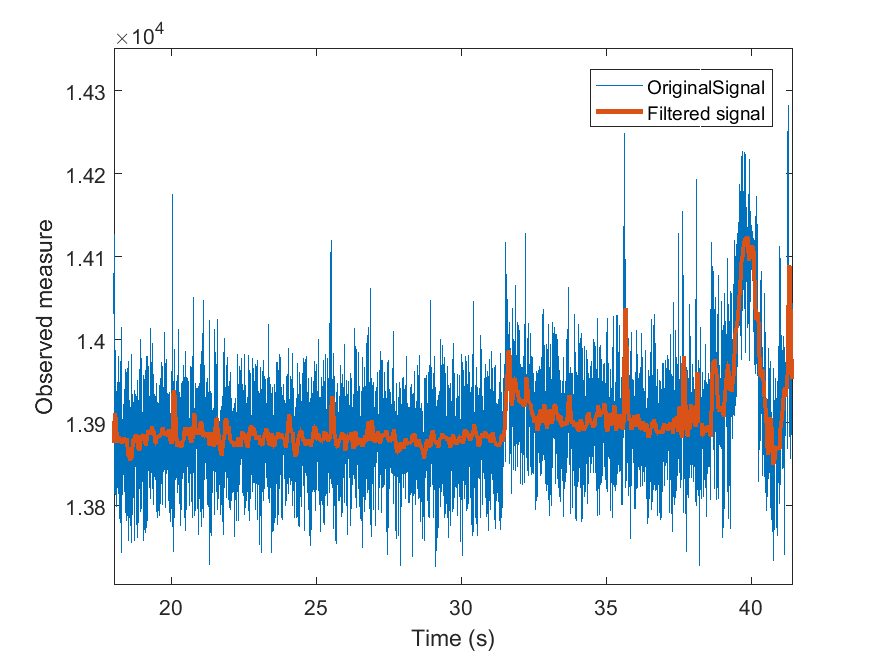
\includegraphics[width=60mm]{pics/ReasonForFailure.png}}
	\subfigure[]{\label{fig:Colours}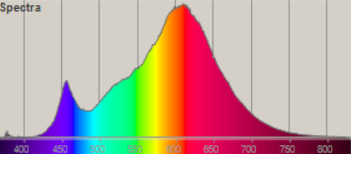
\includegraphics[width=60mm]{pics/Colourspectrum.png}}
	\caption{(a) shows an example of an artefact at $t = 32s$, caused by fluctuations in the power supply. (b) shows the frequency spectrum of the light emitted of the LED used by the system.\label{fig:explanations}}
\end{figure}

\section{Conclusion}
We have developed a method which is capable of analysing a set of consecutive flashes with the goal of detecting bypassing pedestrians, even when a considerable amount of noise sources are mixed in the signal. The created filters and algorithms managed to achieve a combined recall between 0.73 and 0.9 depending on the setting of $T$ and the amount of allowed false positives ratio (0 to 0.05). The system has shown to work on two floors types and on several colours of clothing.

We are aware that the evaluation of the system is minimal, as the system was with a limited dataset. The algorithm was then tweaked by adjusting $T$, to fit the data even more. This method of evaluation at least shows the potential of the system. It also manges to expose some key flaws. It has trouble detecting pedestrians wearing black and blue clothing and has regular false detections if we try to achieve a high detection ratio because of a flaw in the hardware design.

The most direct approach to deal with the identified problems is to improve the hardware design. Changing the LED with one, which emits light more evenly distributed along all wavelengths, will improve the detection ratio of bypassers wearing blue. Changing the power supply and implementing the full system with a detected processor will remove the artefacts and decrease the complexity of the project. It will also allow for the wires to the photodiodes to be shortened and therefore reducing the total amount of noise received by the system.